\section{Stopping muons and protons}
\label{sec:sideband:stopping_muons_protons}

In order to study in detail the reconstruction of the calorimetry, with specific attention to the accuracy of the simulation, detailed high-statistic and fine-binned data/simulation comparisons have been performed.
In a global comparison, discrepancies due to the mis-modelling of \dedx cannot be disentangled from mis-modelling of the underlying kinematic distributions.
Because of this, we realised the importance of comparing distributions of \dqdx or \dedx in fine bins of all relevant variables they depend on.

All the validation plots shown in this section are performed by comparing the \dqdx distribution from the data with the simulation.
The plots are filled once per hit, and they are normalised as follows.
First the beam OFF contributions are subtracted from beam ON events after being normalized to the the number of triggers.
As a second step, the simulation is weighted with the latest GENIE weights, and then area normalised to the data beam ON - beam OFF.

The main purpose of this study is to validate the simulation after applying the re-calibration and test the impact of recombination.
Here we report a subset of the studies that have been performed.
The interested reader can find a complete list of plots of data/simulation comparison in \cite{bib:pid_internal_note}.

\paragraph{Stopping muons at large residual range}
A purely geometrical selection (i.e. without using any calorimetric information) of neutrino-induced stopping muons has been performed, using the following requirements:
\begin{itemize}
    \item Select the longest track in the event
    \item Track length $>$ 30 cm
    \item Track score $>$ 0.5
    \item Track start and end points are required to be contained in a fiducial volume, defined by 20 cm from all TPC borders. The start and end points are corrected for SCE before applying the cut.
    \item Track-vertex distance $<$ 5 cm
    \item Track-muon-momentum-consistency $<$ 0.5. This variable ensures well reconstructed muons, where the range-based-momentum estimate agrees with the multiple-coulomb-scattering (MCS) estimate. The variable is defined as $\displaystyle |p_{\rm range} - p_{\rm MCS}|/p_{\rm range}$
\end{itemize}
This selection achieves a purity of neutrino-induced muons of about 57\%, that becomes 73\% when we subtract the Beam OFF data.

The first validation performed only looks at the MIP-like region of stopping muons, considering only hits at residual range $>$ 30 cm.
This region should show similar data/simulation discrepancies to what was observed with the ACPTs.
Figure \ref{fig:stopping_muons_large_rr_low_pitch} and \ref{fig:stopping_muons_large_rr_high_pitch} show the data/simulation comparisons of the \dqdx distribution before (left) and after (right) re-calibration, in two different bins of pitch and $\phi$.
In both cases there is improvement of the accuracy of the simulation, although it is not complete.
It is noteworthy that the corrections needed in the two angular bins are significantly different, even visually.
This reinforces again the importance of correcting the simulation as a function of the angular variables.

\begin{figure}[H] 
\begin{center}
    \begin{subfigure}[b]{0.45\textwidth}
    \centering
    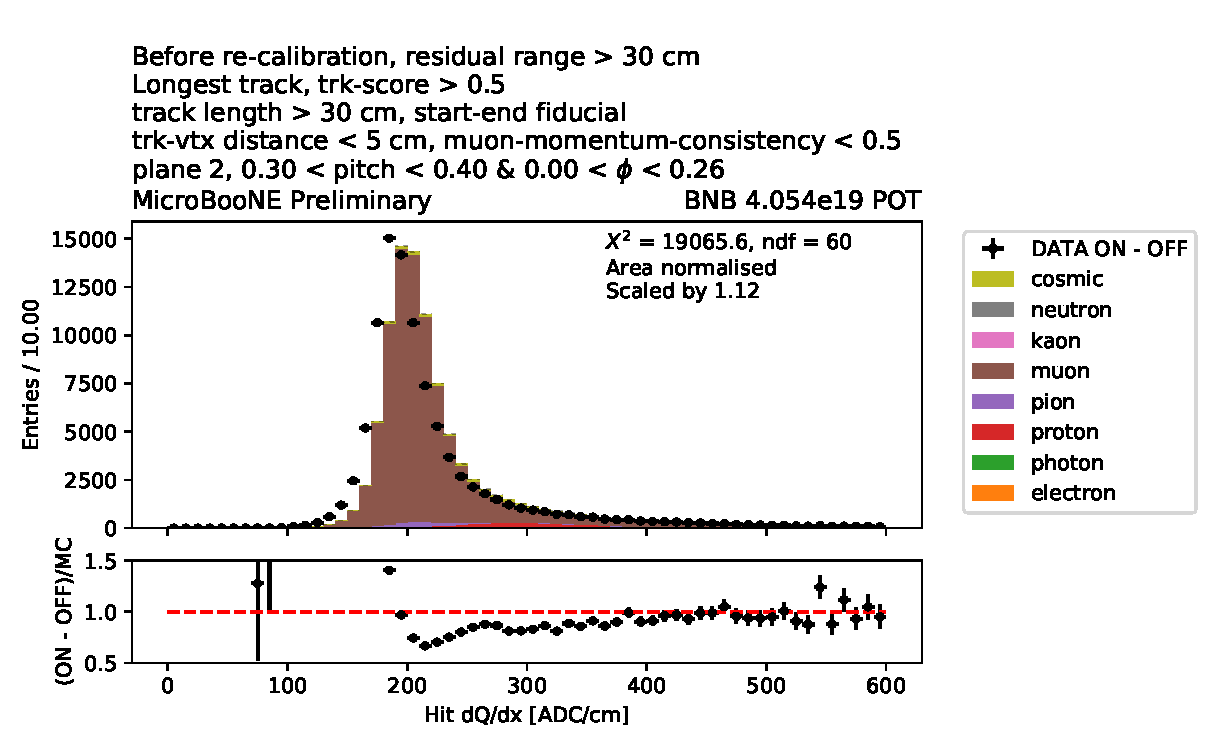
\includegraphics[width=1.00\textwidth]{stopping_muons_protons/030_pitch_040_000_phi_026apres.pdf}
    \end{subfigure}
    \begin{subfigure}[b]{0.45\textwidth}
    \centering
    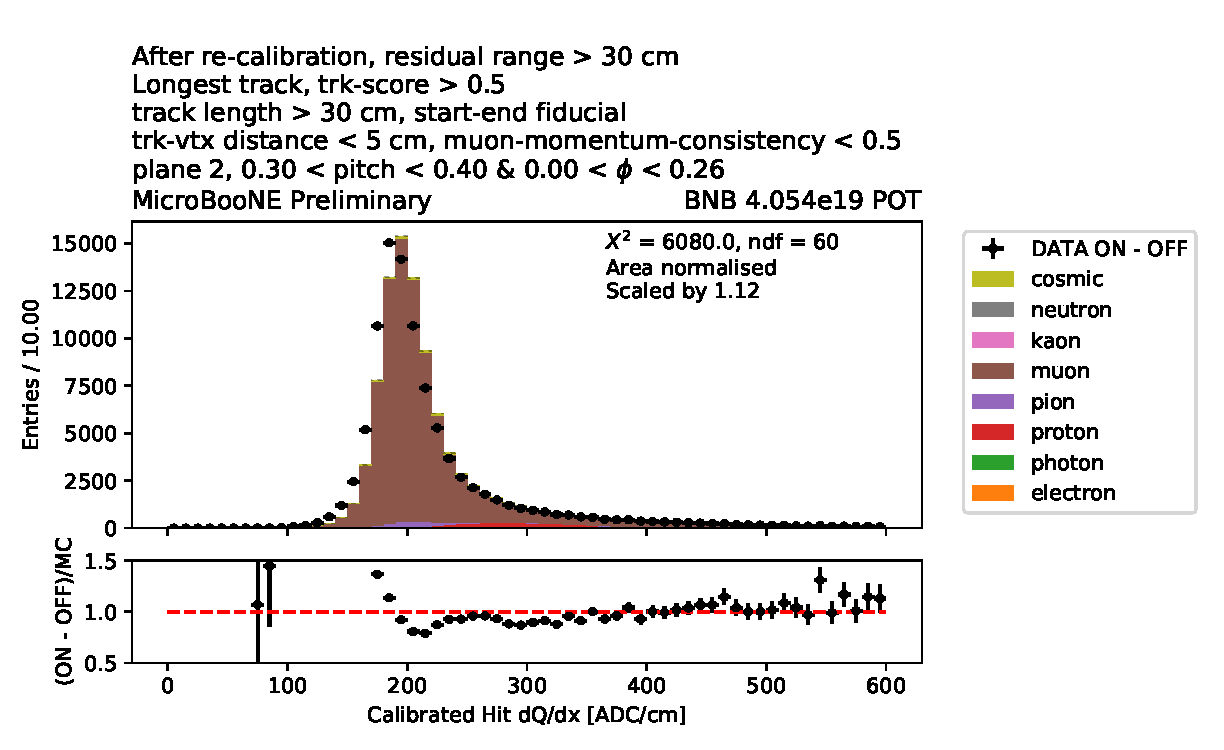
\includegraphics[width=1.00\textwidth]{stopping_muons_protons/030_pitch_040_000_phi_026depois.pdf}
    \end{subfigure}
\caption{Data/simulation comparison of the \dqdx distributions before (left) and after (right) the re-calibration, for stopping muons in the MIP-like region, with residual range $>$ 30 cm, and the bin with 0.3 cm $<$ pitch $<$ 0.4 cm.}
\label{fig:stopping_muons_large_rr_low_pitch}
\end{center}
\end{figure}

\begin{figure}[H] 
\begin{center}
    \begin{subfigure}[b]{0.45\textwidth}
    \centering
    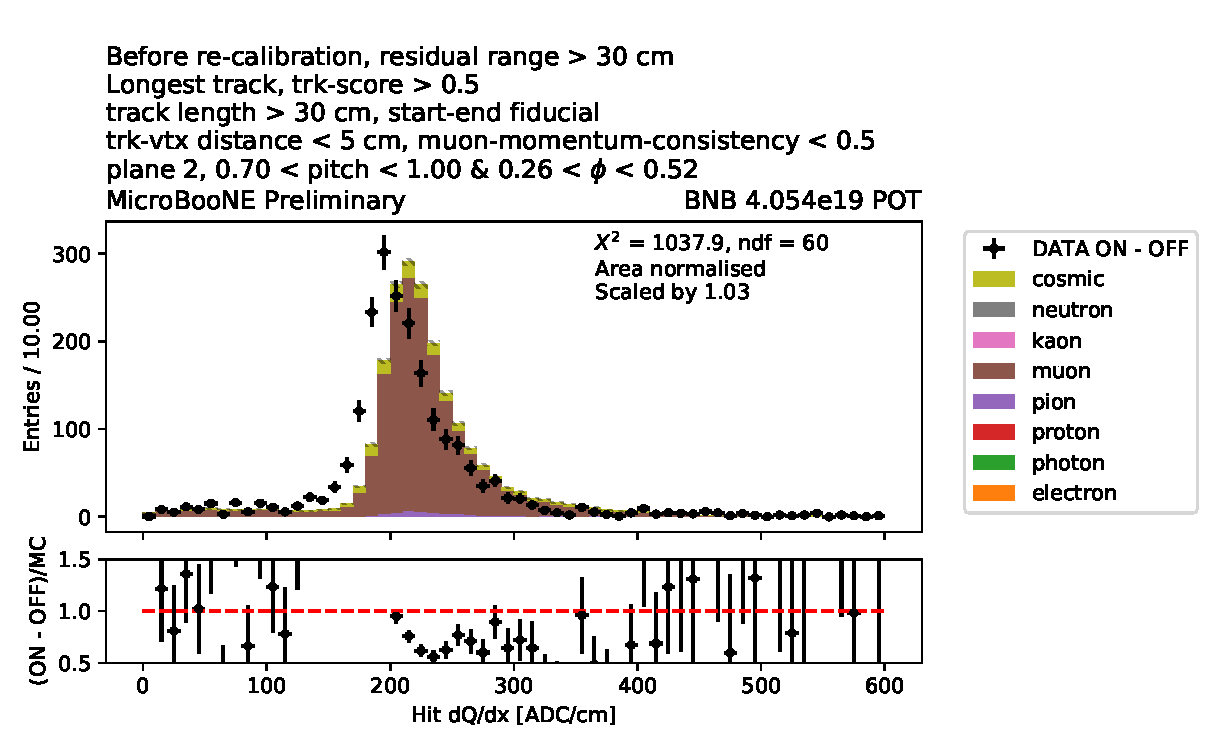
\includegraphics[width=1.00\textwidth]{stopping_muons_protons/070_pitch_100_026_phi_052apres.pdf}
    \end{subfigure}
    \begin{subfigure}[b]{0.45\textwidth}
    \centering
    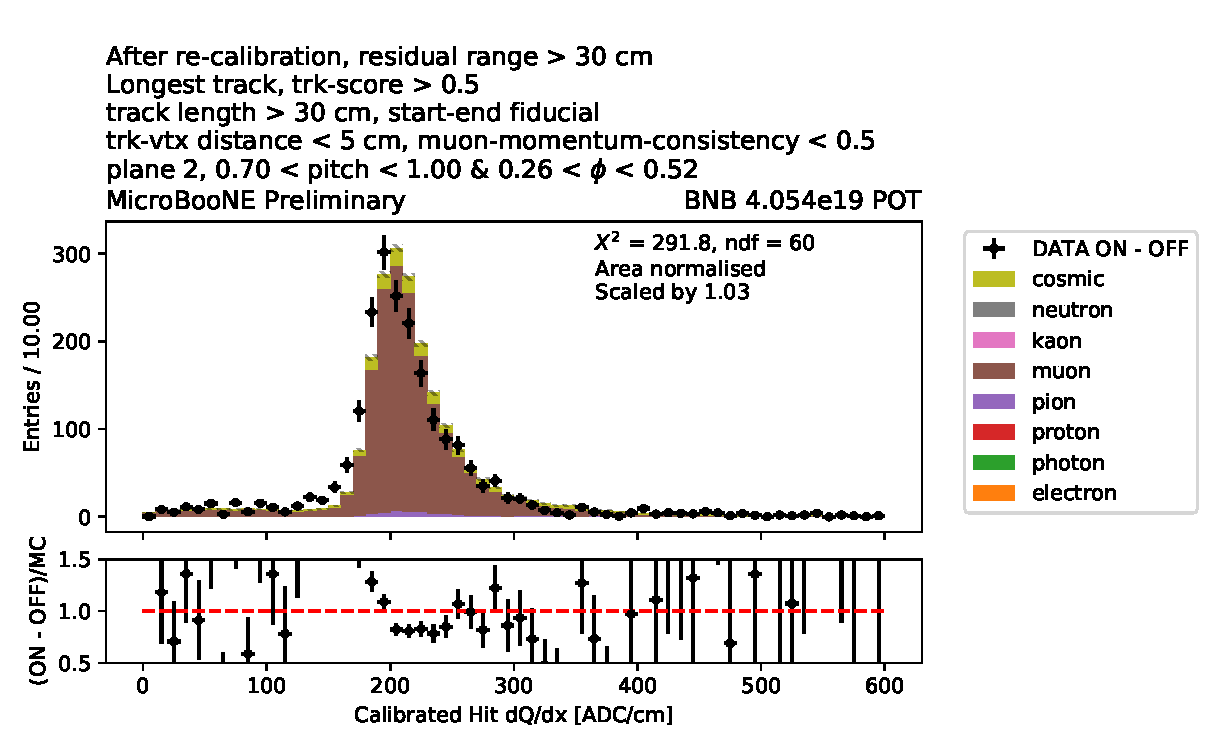
\includegraphics[width=1.00\textwidth]{stopping_muons_protons/070_pitch_100_026_phi_052depois.pdf}
    \end{subfigure}
\caption{Data/simulation comparison of the \dqdx distributions before (left) and after (right) the re-calibration, for stopping muons in the MIP-like region, with residual range $>$ 30 cm, and the bin with 0.7 cm $<$ pitch $<$ 1 cm.}
\label{fig:stopping_muons_large_rr_high_pitch}
\end{center}
\end{figure}

\paragraph{Stopping muons and protons at small residual range}
A second study is performed by looking at stopping muons and protons at low residual range, in order to validate the effect of the re-calibration at larger values of the energy deposition.
In this region data-simulation comparisons are performed in bins of residual range and pitch, before and after applying the correction.
Stopping muons are selected as before, but this time specific bins in residual range are considered, with residual range $<$ 30 cm. 
Stopping protons are selected in data and simulation in the following way:


\begin{itemize}
    \item Track score $>$ 0.5
    \item Track start and end points are required to be contained in a fiducial volume, defined by 20 cm from all TPC borders. The start and end points are corrected for SCE before applying the cut.
    \item Track-vertex distance $<$ 5 cm
    \item Track PID $<$ -0.1
\end{itemize}
This selection achieves a purity of neutrino-induced protons of about 78\%, that becomes 85\% when we subtract the Beam OFF data.
Importantly, this large value of the purity, together with the large value obtained for the muon selection, gives us confidence we are isolating pure samples of particles in a given kinematic region, becoming less and less sensitive to possible mis-modeling of the neutrino interactions.

The two plots in figure \ref{fig:stopping_muons_small_rr_before_after} and \ref{fig:stopping_protons_small_rr_before_after} show the comparisons before (left) and after (right) re-calibration, for stopping muons and protons, respectively.
These studies are performed at small residual range, between 5 cm and 10 cm for the muons, and between 2 cm and 5 cm for the protons.
The pitch is required to be between 0.4 and 1 cm, which is a region where the re-calibration has shown to be effective in the MIP muons.
We can see that in both cases the agreement improves, despite the fact that the simulation does not reproduce all the features of the distribution.

\begin{figure}[H] 
\begin{center}
    \begin{subfigure}[b]{0.45\textwidth}
    \centering
    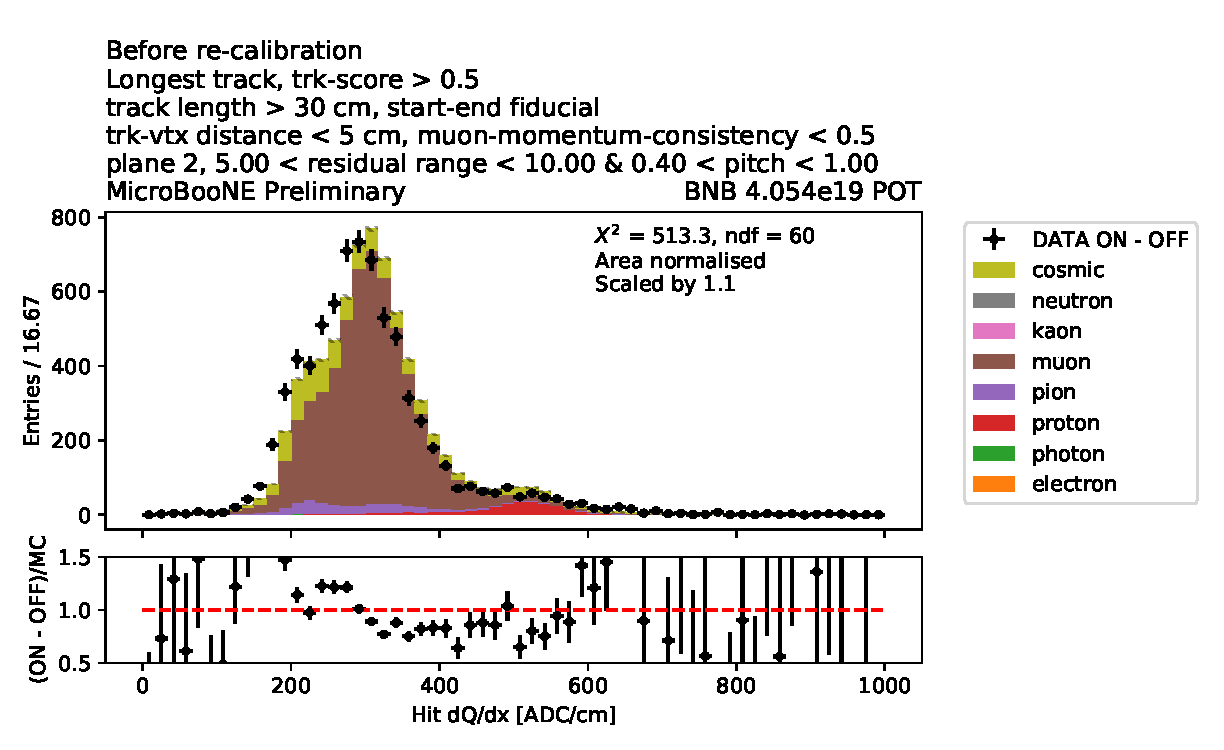
\includegraphics[width=1.00\textwidth]{stopping_muons_protons/muons_500_residualrange_1000_040_pitch_100apres.pdf}
    \end{subfigure}
    \begin{subfigure}[b]{0.45\textwidth}
    \centering
    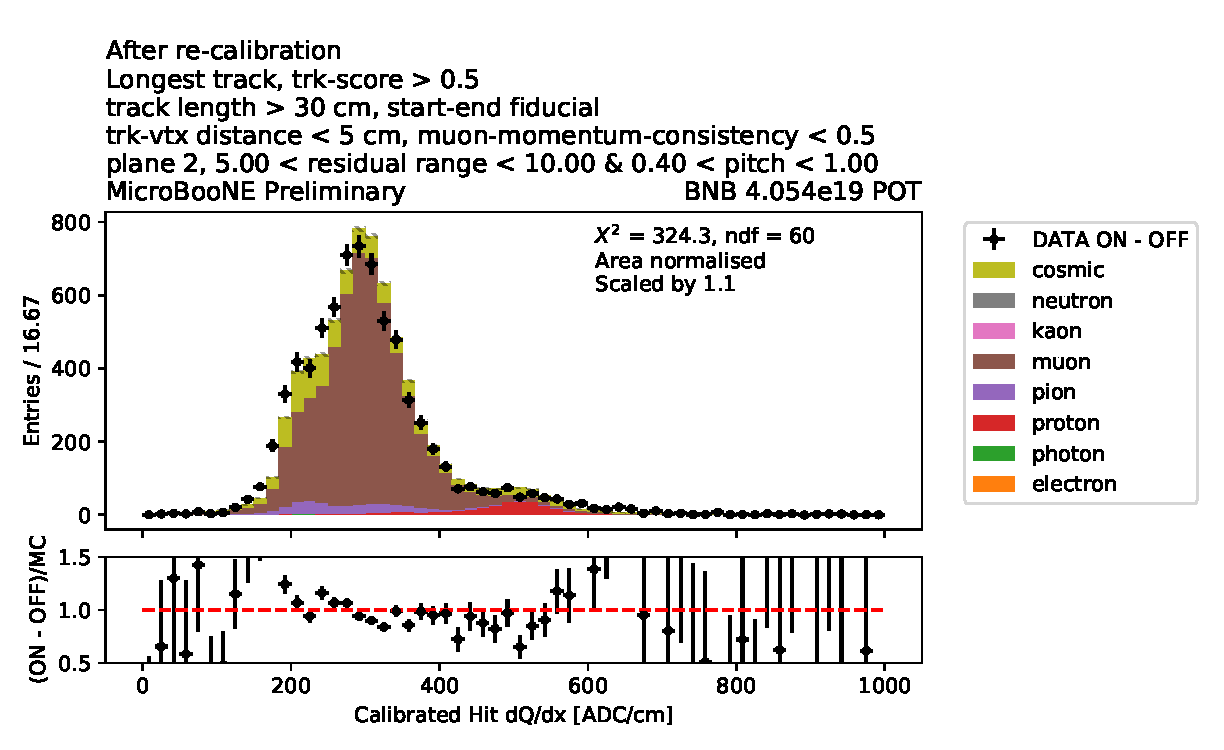
\includegraphics[width=1.00\textwidth]{stopping_muons_protons/muons_500_residualrange_1000_040_pitch_100depois.pdf}
    \end{subfigure}
\caption{Data/simulation comparison of the \dqdx distributions before (left) and after (right) the re-calibration, for stopping muons with residual 5 cm $<$ residual range $<$ 10 cm, and the bin with 0.3 cm $<$ pitch $<$ 0.4 cm.}
\label{fig:stopping_muons_small_rr_before_after}
\end{center}
\end{figure}

\begin{figure}[H] 
\begin{center}
    \begin{subfigure}[b]{0.45\textwidth}
    \centering
    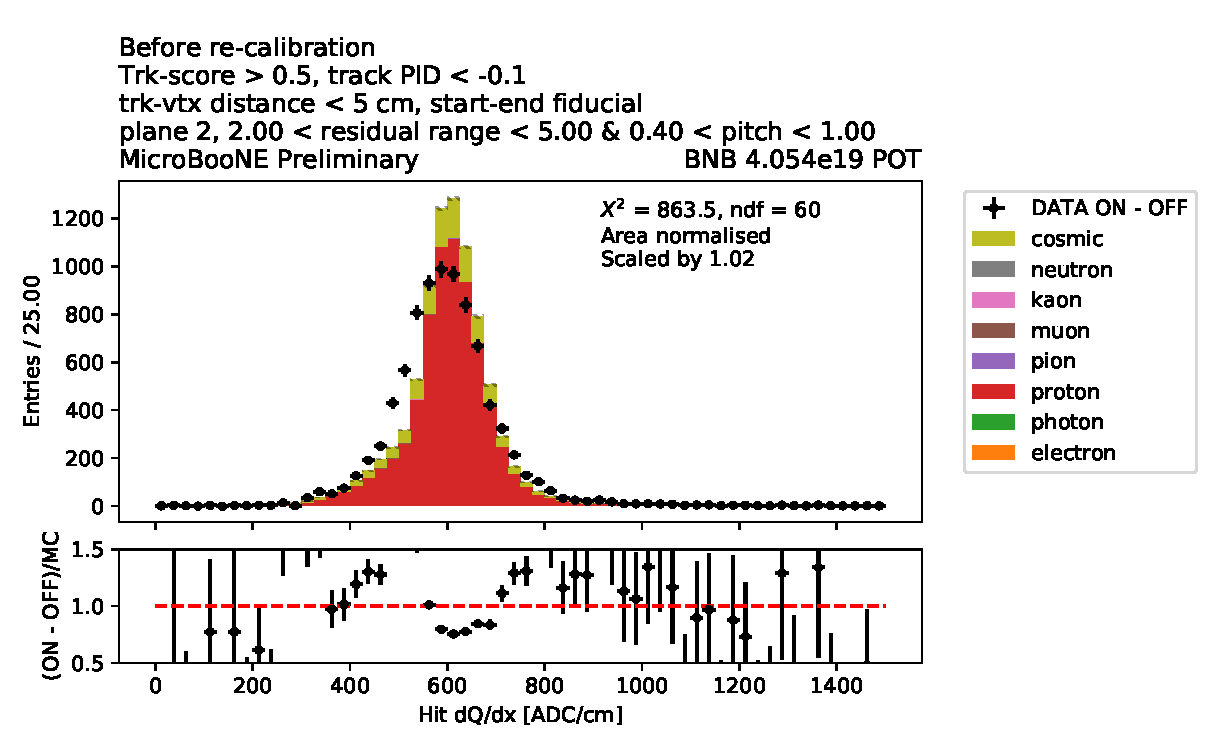
\includegraphics[width=1.00\textwidth]{stopping_muons_protons/protons_200_residualrange_500_040_pitch_100apres.pdf}
    \end{subfigure}
    \begin{subfigure}[b]{0.45\textwidth}
    \centering
    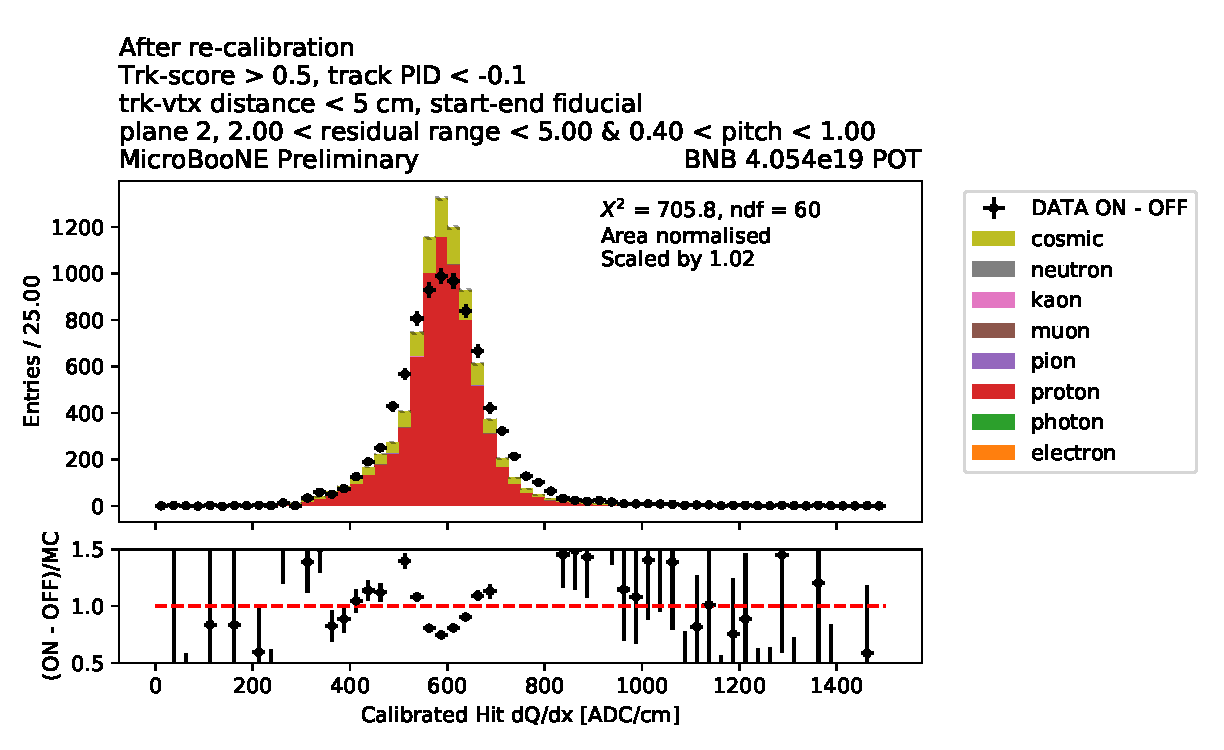
\includegraphics[width=1.00\textwidth]{stopping_muons_protons/protons_200_residualrange_500_040_pitch_100depois.pdf}
    \end{subfigure}
\caption{Data/simulation comparison of the \dqdx distributions before (left) and after (right) the re-calibration, for stopping protons with residual 2 cm $<$ residual range $<$ 5 cm, and the bin with 0.4 cm $<$ pitch $<$ 1 cm.}
\label{fig:stopping_protons_small_rr_before_after}
\end{center}
\end{figure}

\paragraph{Effect of recombination}
In order to study how well the effect of recombination is simulated, it is very useful to look at protons at very small residual range.
In order to disentangle recombination from detector effects, the following plots are restricted to the region at small pitch, between 0.3 and 0.4 cm.
The four plots shown in Figures \ref{fig:stopping_muons_recombination} and \ref{fig:stopping_protons_recombination} show the comparisons, after the re-calibration, for stopping protons with residual range between 0 and 2 cm, 2 and 5 cm, 5 and 10 cm, and 10 and 20 cm, respectively.

No substantial non-linear effect in the calibration is present.
This is confirmed also by the good agreement between the data and the theory seen in Figure \ref{fig:llr_pid_pdf_example}.

We believe the simulation, although not perfect, reproduces all features observed in the data, and it is thus good enough for the rest of the analysis.

The studies shown in this section after the re-calibration, while showing residual data/simulation discrepancies limited to specific regions of the phase space, give us confidence in having reached a level of detector modeling adequate for the successful performance of this analysis. 
The impact of detector mis-modeling is further evaluated in terms of the systematic impact of detector effects in \ref{sec:detsys}.

\begin{figure}[H] 
\begin{center}
    \begin{subfigure}[b]{0.45\textwidth}
    \centering
    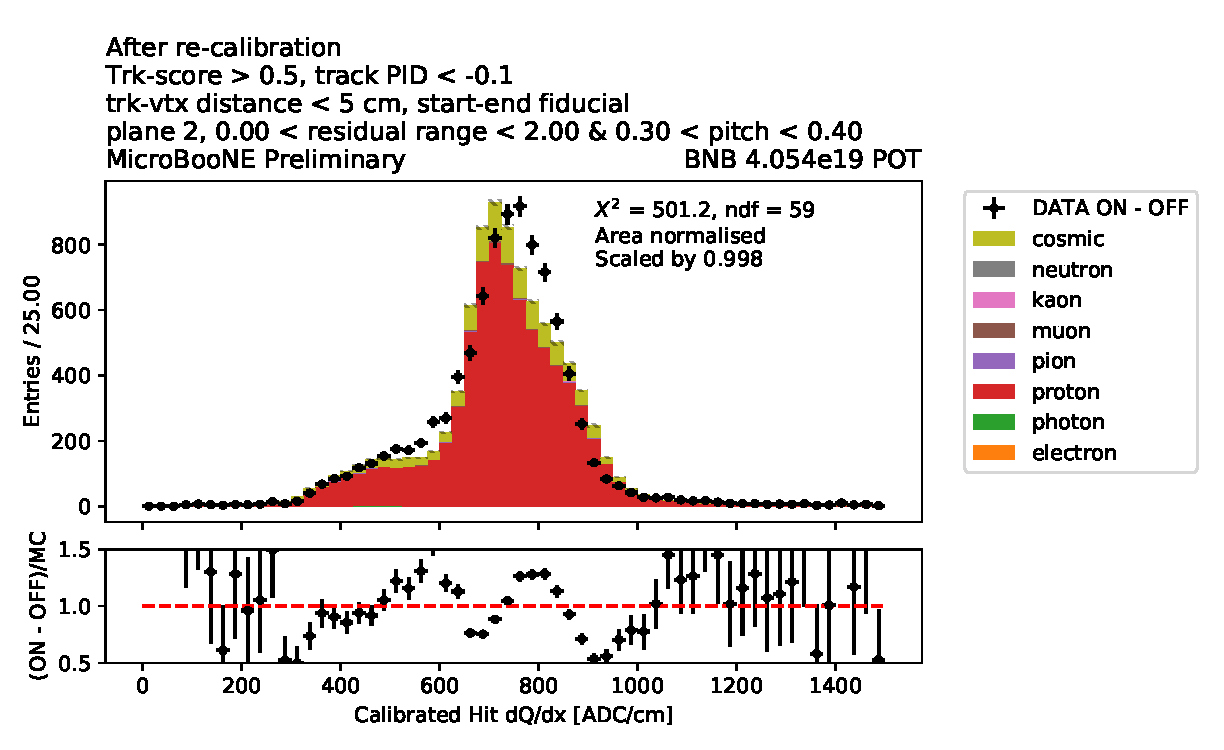
\includegraphics[width=1.00\textwidth]{stopping_muons_protons/protons_000_residualrange_200_030_pitch_040depois.pdf}
    \end{subfigure}
    \begin{subfigure}[b]{0.45\textwidth}
    \centering
    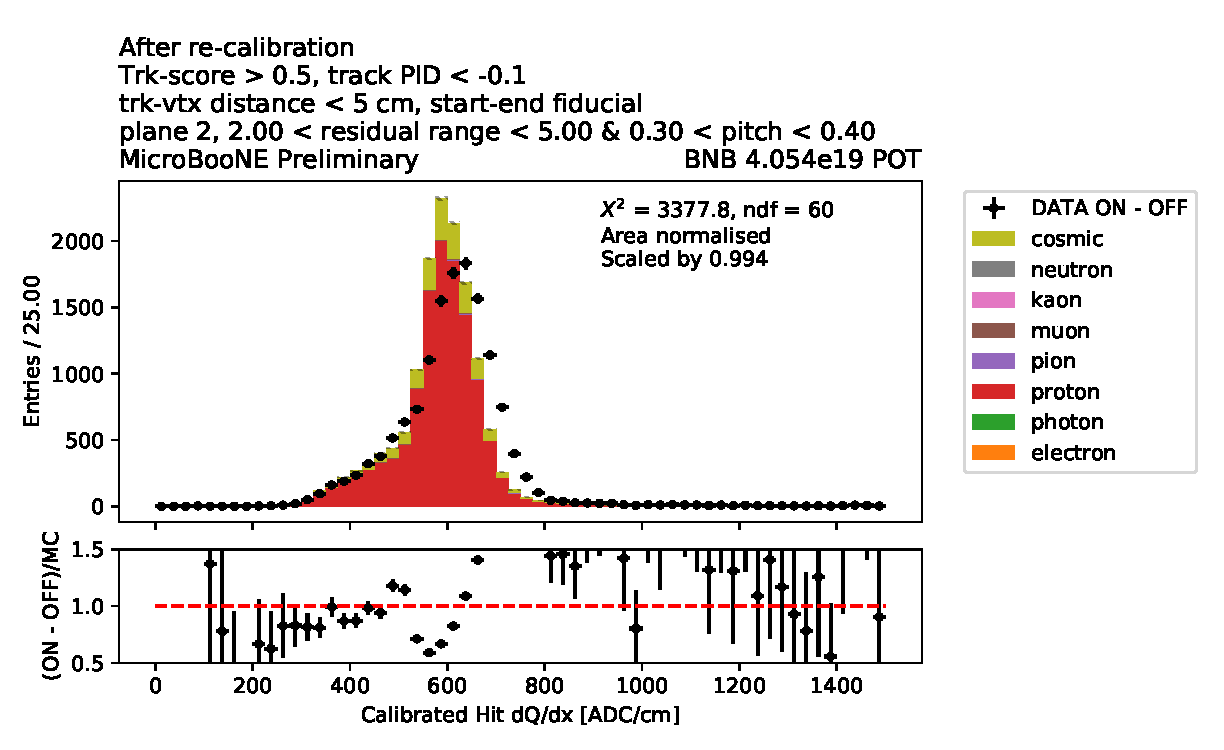
\includegraphics[width=1.00\textwidth]{stopping_muons_protons/protons_200_residualrange_500_030_pitch_040depois.pdf}
    \end{subfigure}
\caption{Data/simulation comparison of  \dqdx after the re-calibration, for stopping protons with 0.3 cm $<$ pitch $<$ 0.4 cm and 0 cm $<$ residual range $<$ 2 cm (left plot), and 2 cm $<$ residual range $<$ 5 cm (right plot).}
\label{fig:stopping_muons_recombination}
\end{center}
\end{figure}

\begin{figure}[H] 
\begin{center}
    \begin{subfigure}[b]{0.45\textwidth}
    \centering
    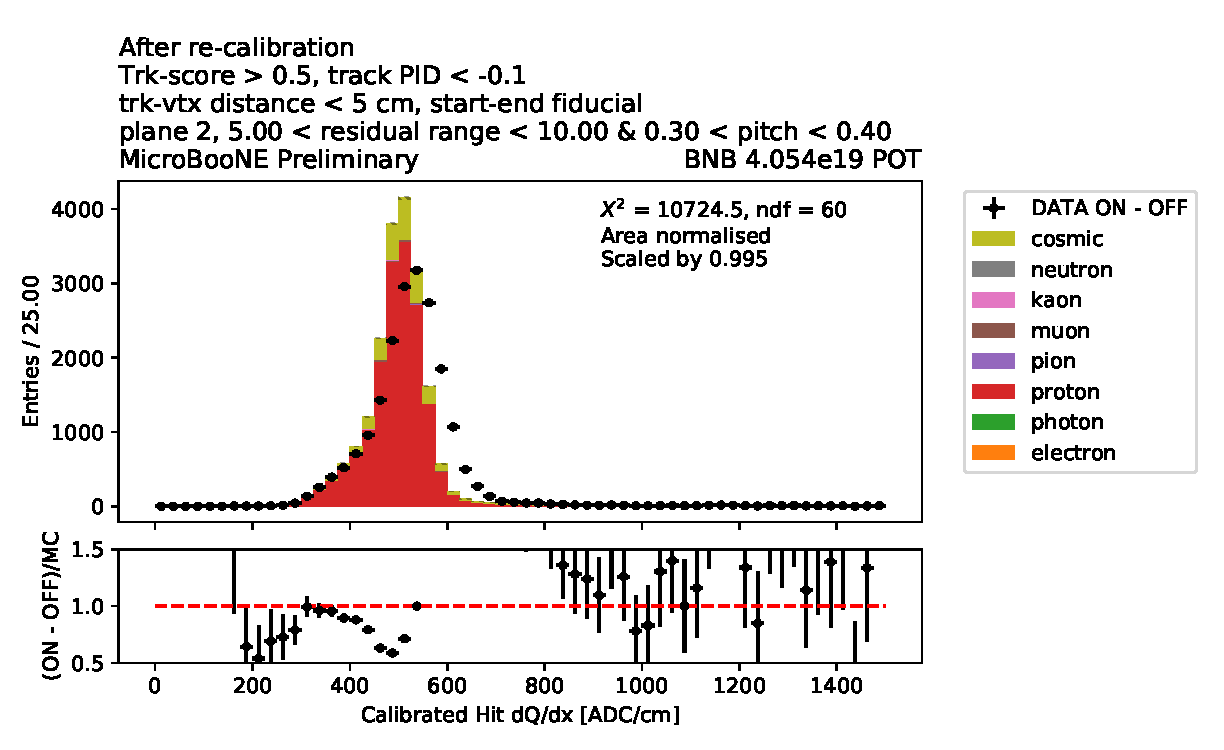
\includegraphics[width=1.00\textwidth]{stopping_muons_protons/protons_500_residualrange_1000_030_pitch_040depois.pdf}
    \end{subfigure}
    \begin{subfigure}[b]{0.45\textwidth}
    \centering
    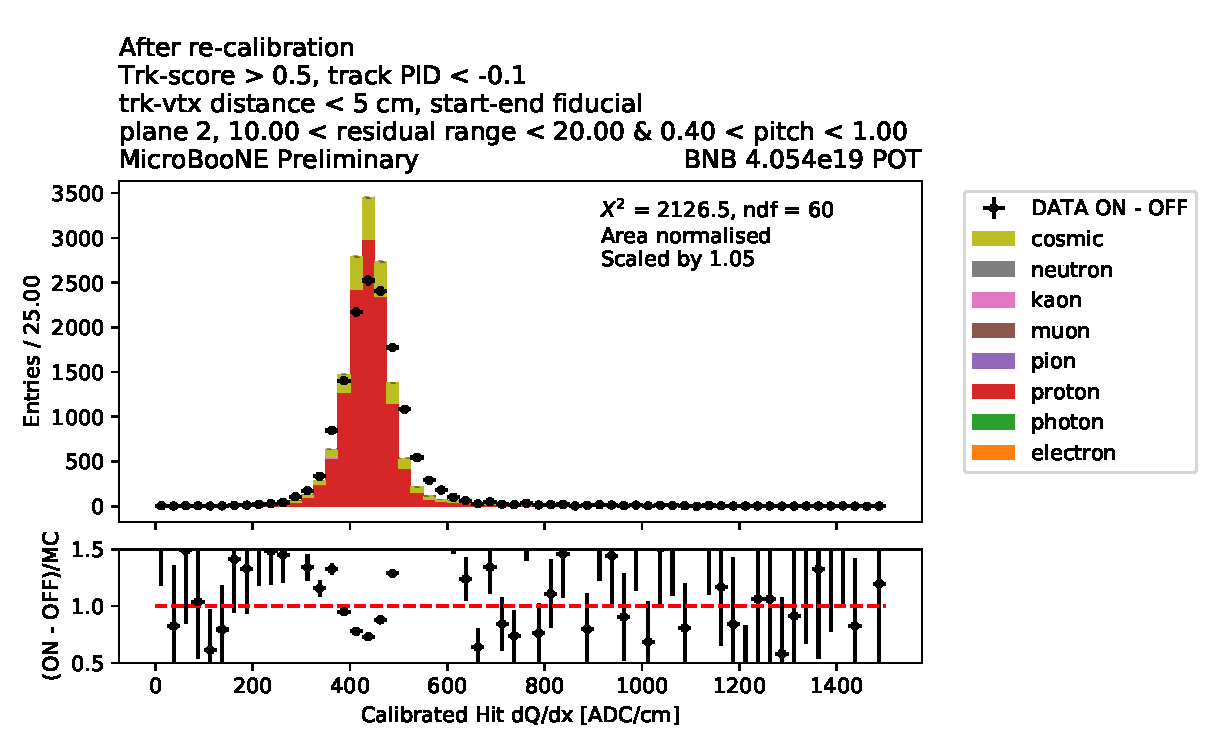
\includegraphics[width=1.00\textwidth]{stopping_muons_protons/protons_1000_residual_range_2000_040_pitch_100depois.pdf}
    \end{subfigure}
\caption{Data/simulation comparison of \dqdx after the re-calibration, for stopping protons with 0.3 cm $<$ pitch $<$ 0.4 cm and 5 cm $<$ residual range $<$ 19 cm (left plot), and 10 cm $<$ residual range $<$ 20 cm (right plot).}
\label{fig:stopping_protons_recombination}
\end{center}
\end{figure}
\paragraph{Limitations}
Despite the good degree of accuracy, we realise that the current calorimetric reconstruction and the methods developed in this analysis contain several limitations.

As previously observed, in certain bins the re-calibration only corrects the scale of the distribution, lacking of an additional smearing.
Additionally, the re-calibration applied to neutrino-induced particles is in general not as effective as on the ACPTs.
We have seen that the scale of the distribution is still not accurate even after the re-calibration, and in certain bins, the correction even goes in the opposite direction with respect to the discrepancy.
We understood these effects are related, at least partially, to the coarseness of the bins in which the re-calibration is computed.
With coarse bins, the difference between ACPTs and neutrino-induced particles in the angular distributions in every single bin become relevant, producing calibration factors which are not very accurate for the neutrino induced particles.

All these studies have been documented in detail in \cite{bib:pid_internal_note}, which contains all data/simulation comparisons in all bins of phase space.
